\section{Key-Takeaways}

Access this document online: \url{https://v2.overleaf.com/read/pnfhvvbbzxfc}
Or access it by clicking \href{https://v2.overleaf.com/read/pnfhvvbbzxfc}{here}.

\begin{itemize}
    \item Extra spaces      do not appear. \\
        Start typing after tabs.
    \item Insert and re-scale a image.

        \begin{figure}[ht] % ht: here, top
        \centering
        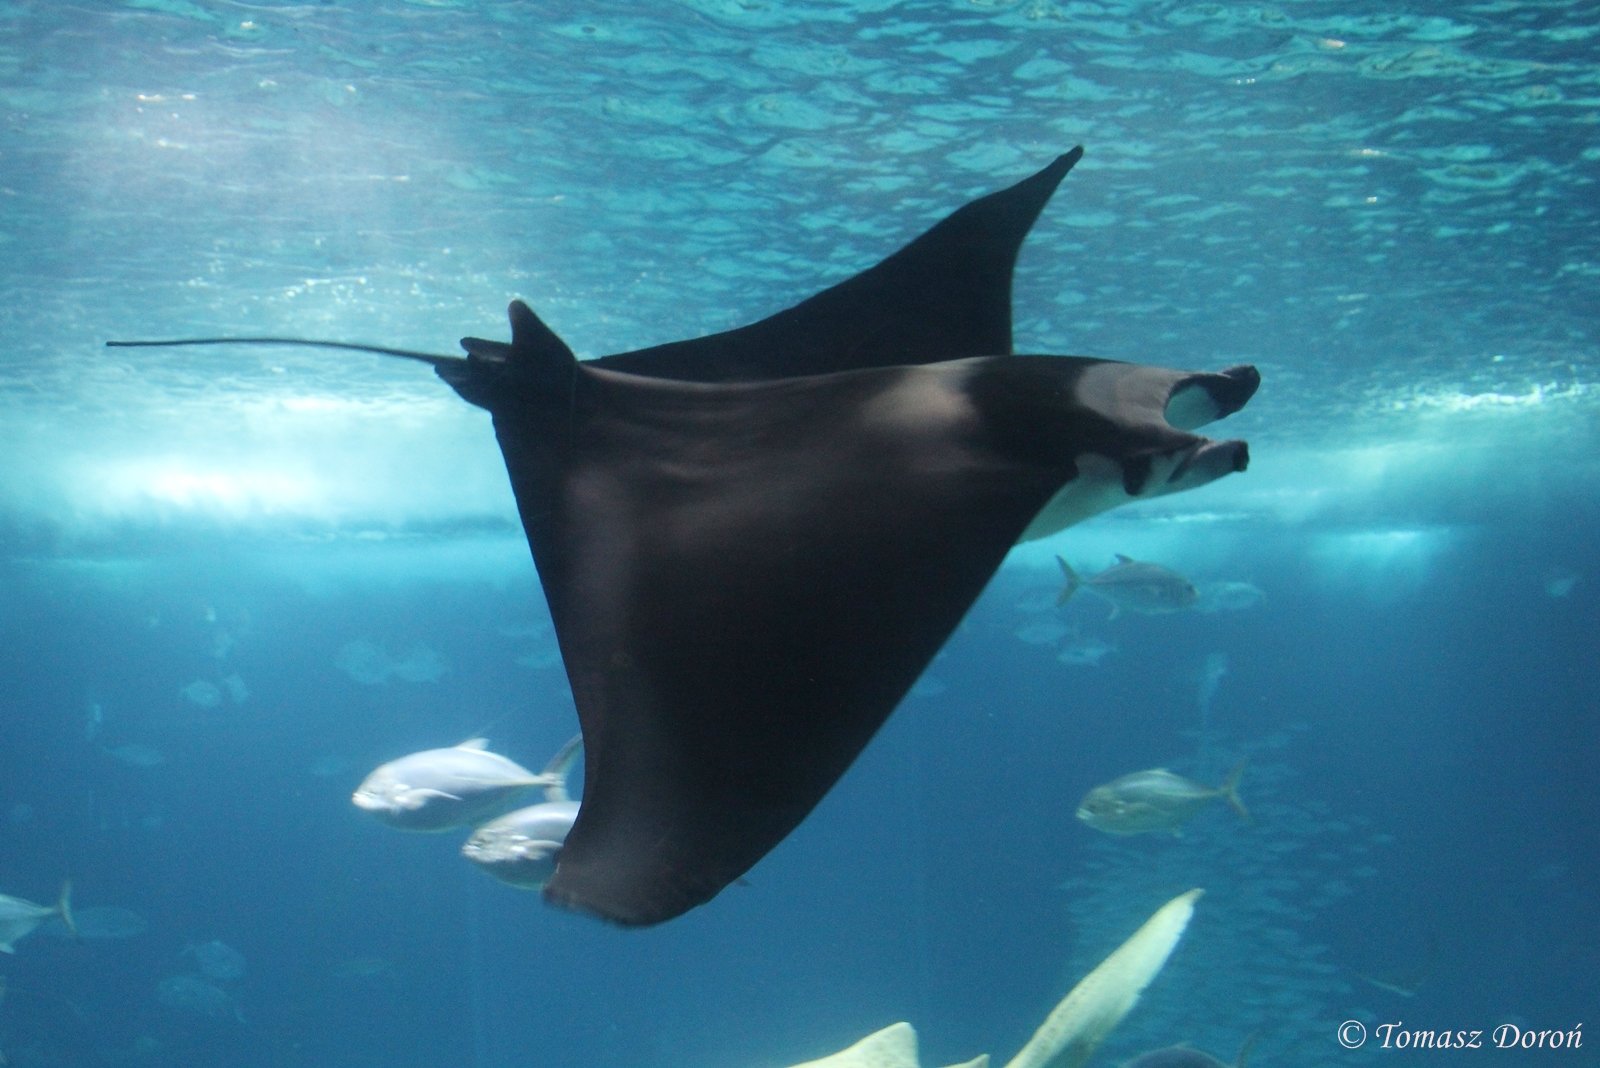
\includegraphics[width=8cm,height=5 cm]{DevilRay.JPG} % try  Scale the picture with [scale = 0.4][width=\textwidth]
        \caption{Look! I can fly.}
        \label{fig:my_DevilRay}
        \end{figure}

        Here is some text after my image.
    \item un-ordered shopping-list

        \begin{itemize}
            \item milk,
            \item banana,
            \item soap,
        \end{itemize}  
    
    \item ordered list:
        \begin{enumerate}
            \item chocolate,
            \item soap,
                \begin{enumerate}
                    \item must be bar soap,
                    \item prefer Dove brand.
                \end{enumerate}
            \item milk.
    \end{enumerate}
    
    \item Why the Devil-Ray is the best choice? 
    \footnote{9 Facts About Devil Rays - \url{http://www2.padi.com/blog/2015/10/31/9-facts-about-devil-rays/}}
 
    \begin{itemize}
    

 
        \item they have been around for 20-25 million years.
        
        \item the deepest, fastest divers in the ocean. (Devil rays can dive to depths of nearly 2km for around 60-90 minutes, at speeds of 13mph or 22km/h.)
        
        \item Devil rays are actually harmless, shy creatures and filter-feed on...
        
        \begin{enumerate}
            \item plankton,
            \item krill,
            \item small fish.
            
        \end{enumerate}
    \end{itemize}
    
    \item Formatting
    \begin{flushright} This text is right justified.
    \end{flushright}
    \begin{center} Centered text.
    \end{center}

Return to paragraph mode.

Here is some \textbf{bold text}.\\
Now for some \textit{italic font}.\\
\emph{Here is some  \emph{emphasized text.}}

This is {\large a bit larger} text.\\
Slightly {\Large bigger} text.\\
Even {\LARGE bigger} again.\\
Now for some {\small small} text.

    \item Keep typing on the next page.
    
    \item Symbols
    
    There is a 40\% chance of rain today.
    I like cats \& dogs.\\
    To type backslash using a special command: \textbackslash 
    
    Batman symbol: \Bat
    
    My friend's name is \AA Shild. \cite{mittelbach2004latex}
    
{\Huge    We are learning \LaTeX}

    \item Tables

\vspace{1cm}
    
    \item Math-modes
    
    \item Citation and Reference
    
\end{itemize}